% CVPR 2022 Paper Template
% based on the CVPR template provided by Ming-Ming Cheng (https://github.com/MCG-NKU/CVPR_Template)
% modified and extended by Stefan Roth (stefan.roth@NOSPAMtu-darmstadt.de)

\documentclass[10pt,twocolumn,letterpaper]{article}

%%%%%%%%% PAPER TYPE  - PLEASE UPDATE FOR FINAL VERSION
\usepackage[review]{cvpr}      % To produce the REVIEW version
%\usepackage{cvpr}              % To produce the CAMERA-READY version
%\usepackage[pagenumbers]{cvpr} % To force page numbers, e.g. for an arXiv version

% Include other packages here, before hyperref.
\usepackage{graphicx}
\usepackage{amsmath}
\usepackage{amssymb}
\usepackage{booktabs}
\usepackage{cite}
\usepackage{algorithmic}
\usepackage{textcomp}
\usepackage{xcolor}
\usepackage{graphicx} % for \includegraphics command
\usepackage{float} % for [H] option to force figure placement
\usepackage{caption}
\usepackage{booktabs}
\usepackage{multirow}
\usepackage{animate}
\usepackage[colorlinks=true, linkcolor=blue, urlcolor=blue]{hyperref}
\def\BibTeX{{\rm B\kern-.05em{\sc i\kern-.025em b}\kern-.08em
    T\kern-.1667em\lower.7ex\hbox{E}\kern-.125emX}}


% It is strongly recommended to use hyperref, especially for the review version.
% hyperref with option pagebackref eases the reviewers' job.
% Please disable hyperref *only* if you encounter grave issues, e.g. with the
% file validation for the camera-ready version.
%
% If you comment hyperref and then uncomment it, you should delete
% ReviewTempalte.aux before re-running LaTeX.
% (Or just hit 'q' on the first LaTeX run, let it finish, and you
%  should be clear).
\usepackage[pagebackref,breaklinks,colorlinks]{hyperref}


% Support for easy cross-referencing
\usepackage[capitalize]{cleveref}
\crefname{section}{Sec.}{Secs.}
\Crefname{section}{Section}{Sections}
\Crefname{table}{Table}{Tables}
\crefname{table}{Tab.}{Tabs.}


%%%%%%%%% PAPER ID  - PLEASE UPDATE
\def\cvprPaperID{*****} % *** Enter the CVPR Paper ID here
\def\confName{CVPR}
\def\confYear{2022}


\begin{document}

%%%%%%%%% TITLE - PLEASE UPDATE
\title{Answering Queries in Egocentric Videos: an Integrated Approach using Natural Language Localization and Visual Language Model}

\author{Cecilia Berti\\
Politecnico di Torino\\
{\tt\small s328490@studenti.polito.it}
\and
Alessia Manni\\
Politecnico di Torino\\
{\tt\small s331377@studenti.polito.it}
\and
Shakti Rathore\\
Politecnico di Torino\\
{\tt\small s328222@studenti.polito.it}
}

\maketitle

%%%%%%%%% ABSTRACT
\begin{abstract}
In this paper, we address the challenge of localizing relevant video segments in response to natural language queries and subsequently generating corresponding textual answers.  We present a pipeline that combines two specialized models for different phases of the workflow. Natural Language Video Localization (NLVL) involves locating a matching span from the video that semantically corresponds to the query, for this task we deploy VSLNet, an enhanced version of the VSLBase architecture. VSLNet relies on a multi-modal approach that integrates visual and textual information, producing the temporal boundaries of the relevant video segment. The key element of VSLNet is its Query-Guided Highlighting (QGH) component, which guides the search for matching video segments within a highlighted region, leading to more accurate localization. For the task of generating answers, we deploy a novel Large Vision-Language model, Video LLaVA, which extends the capabilities of large vision-language models to understand both images and videos. This model processes the textual query along with the shortened video, which has been clipped according to the previously predicted boundaries. Video LLaVa integrates visual representations into the textual feature space, enabling the large language model (LLM) to generate effective textual answers. We evaluate our approach on the Ego4D dataset, demonstrating robust performance through both quantitative and qualitative assessments. The code is available at \href{https://github.com/Gin549/episodic-memory-pers}{https://github.com/Gin549/episodic-memory-pers}.
\end{abstract}

\section{Introduction}
In recent years, the scientific focus has shifted towards the next generation of mobile computing—wearable devices. This shift has spurred significant advancements in egocentric vision. Among its various applications, first-person or “egocentric” perception using wearable cameras has the potential to alleviate cognitive overload and provide users with a superhuman personal episodic memory. By capturing and indexing what we see in meaningful and easily accessible ways, these devices could transform how we interact with our environment.

This purpose is embodied by the Natural Language Query (NLQ) task in the Ego4D Episodic Memory benchmark. The NLQ challenge involves taking a natural language query and a video clip, and identifying the exact temporal segment in the camera wearer's past footage that contains the answer \cite{b1}. These types of problems are referred to as Natural Language Video Localization (NLVL) problems.

The task can be approached in two ways: as a video segment matching problem, where the goal is to find the best matching segment given a query \cite{b2}, or as a regression problem, which directly predicts the boundaries of the relevant video segment \cite{b3}.

The NLQ challenge, along with related video-language question answering tools, has gained considerable attention from the research community. However, the task presents several technical challenges. Firstly, videos may be of arbitrary length, which raises the question of how to build models that can reason over a long temporal range. Secondly, integrating video and text modalities remains a complex issue.

In this paper, we propose an approach that first solves the NLVL problem by extracting the start and end boundaries of the answer span from the video. Then, we exploit a Large Language Visual Model to generate a natural language answer from the extracted clip.

As a baseline, we first address the NLVL task with a standard span-based QA framework for video input named VSLBase, whose architecture is presented in section 4, comparing the outcomes obtained using different sets of pre-extracted features. We then propose an improved version, VSLNet, implemented with different encoders to assess the most effective version. Finally, we utilize an open-source model, Video-LLaVA, detailed in section 5B. This model generates natural language answers to the posed questions, which are then evaluated both quantitatively and qualitatively.

\section{Related work}

\subsection{Localizing Video Segments with Natural Language}

The task of localizing moments within a long video has improved enormously in the last few years. Prior work was solely based on scanning videos by predefined windows of different sizes. Gao et al. (2017) introduced the first dataset, "TACoS," for temporal activity localization with sentence descriptions, utilizing a sliding window approach. These methods typically generate segment candidates throughout the video using temporal sliding windows. These segments are then either compared (Hendricks et al. 2017) or combined (Gao et al. 2017) with the given sentence to identify the relevant parts of the video. While these models achieve good overall matching between video segments and sentences, they often miss fine-grained interactions and context details, and are inefficient due to the exhaustive search process across the video's timeline, making them computationally expensive \cite{b4}.


To address the challenges related to context understanding, Zhang et al.(2020), proposed TAN-2D model. The goal was to localize the target moment on a two-dimensional map that captures the relationship between a specific moment and all other temporal segments. The main idea behind the model is that after extracting features from the moment candidates within the video, these features are organized into a 2D temporal feature map. The next part involves multi-modal fusion with textual features, followed by the application of a Temporal Adjacent Network on the fused feature map to enhance the model's contextual awareness of adjacent moments.

In this paper, we closely follow the model proposed by Hao et al. in \cite{b3}, which treats the input video as a text passage, transforming NLVL into a standard span-based QA problem. VSLBase adopts a simple and standard span-based QA framework, facilitating the modeling of differences between video and text through the addition of extra modules. The VSLNet addresses these differences by introducing the QGH module.



\subsection{Large Language Visual Models}
Recent advancements in natural language processing have extended the capabilities of large language models (LLMs) to comprehend not only textual data but also visual content. One notable approach involves mapping images into text-like tokens, which allows LLMs to process both text and images in a unified manner. This integration of visual and textual information enables LLMs to understand and generate responses based on visual input.

Several of these new architectures leverage pre-trained large language models to build unified models for multi-modality. For instance, Flamingo [Alayrac et al., 2022] employs a frozen vision encoder and large language model, using gated cross-attention to fuse vision and language modalities, demonstrating impressive few-shot capabilities. BLIP-2 [Li et al., 2023] introduces Q-Former to align visual features from the frozen visual encoder with large language models.

In this paper, we examine Video-LLaVA, a robust baseline for LLVM that manages both images and videos simultaneously. Like MiniGPT-4 \cite{b6}, Video-LLaVA pre-aligns image and video features, but also conducts joint training of images and videos, enabling LLMs to develop multi-modal reasoning capabilities from a unified visual representation.

Despite their strengths, these models face limitations due to their reliance on frozen visual backbones, which may result in suboptimal alignment because of the restricted parameter set. To address these shortcomings, mPLUG-Owl \cite{b7} has been introduced. This model not only aligns representations between vision and language foundation models for enhanced knowledge acquisition and real-world grounding but also excels in understanding language and multi-modal instructions.


\section{Dataset}
Traditional computer vision systems have relied on third-perspective images for a very long time. Addressing this limitation, the Ego4D dataset represents a revolutionary leap in the field of first-person visual perception. Ego4D comprises of a total of 3670 hours of egocentric video footage captured by 931 different participants across 74 locations worldwide. This dataset, created by Facebook AI (now Meta AI) in collaboration with numerous academic institutions and research organizations, is the most diverse and curated collection of daily-life activities to date, including household chores, leisure activities, work tasks and more. 

To mitigate overfitting, Ego4D employs seven different head-mounted cameras, capturing a broader spectrum of human behavior and interactions than previous datasets. Additionally, it introduces five benchmark challenges aimed at testing and enhancing AI systems' capabilities in first-person perception. 

Our focus is on the Episodic memory challenge, which aims to evaluate and advance AI systems’ capabilities to understand and recall past events from egocentric video data. Specifically, it addresses queries expressed in natural language, with responses providing temporal windows for observing or inferring answers. To approach this task, the dataset provides extensive annotations which include:
\begin{itemize}
\setlength{\parskip}{0.05cm}   

    \item \textbf{Detailed timestamps}: since in ego4d videos are divided into shorter segments called clips, annotations specify start and end timestamps for segments within individual video clips and in relation to the entire video.
    \item \textbf{Language queries}: Each annotation includes formulated questions aimed at extracting specific information from the video content.
    \item \textbf{Temporal information}: Queries are accompanied by temporal data indicating their occurrence within both the clip and the overall video, along with the “response track” in the video.
    \item \textbf{Template descriptions}: Annotations provide a set of 13 template questions, with designated slots for variables (X, Y) such as objects and actions, meant to span things a user might ask to augment their memory. In fig. \ref{fig:figure1} we report the distribution of queries per template.
    \item \textbf{Raw tags}: Included to capture the essence of the queries, aiding in processing and analysis of the annotated data.

\end{itemize}

\begin{figure}[h]
\centering
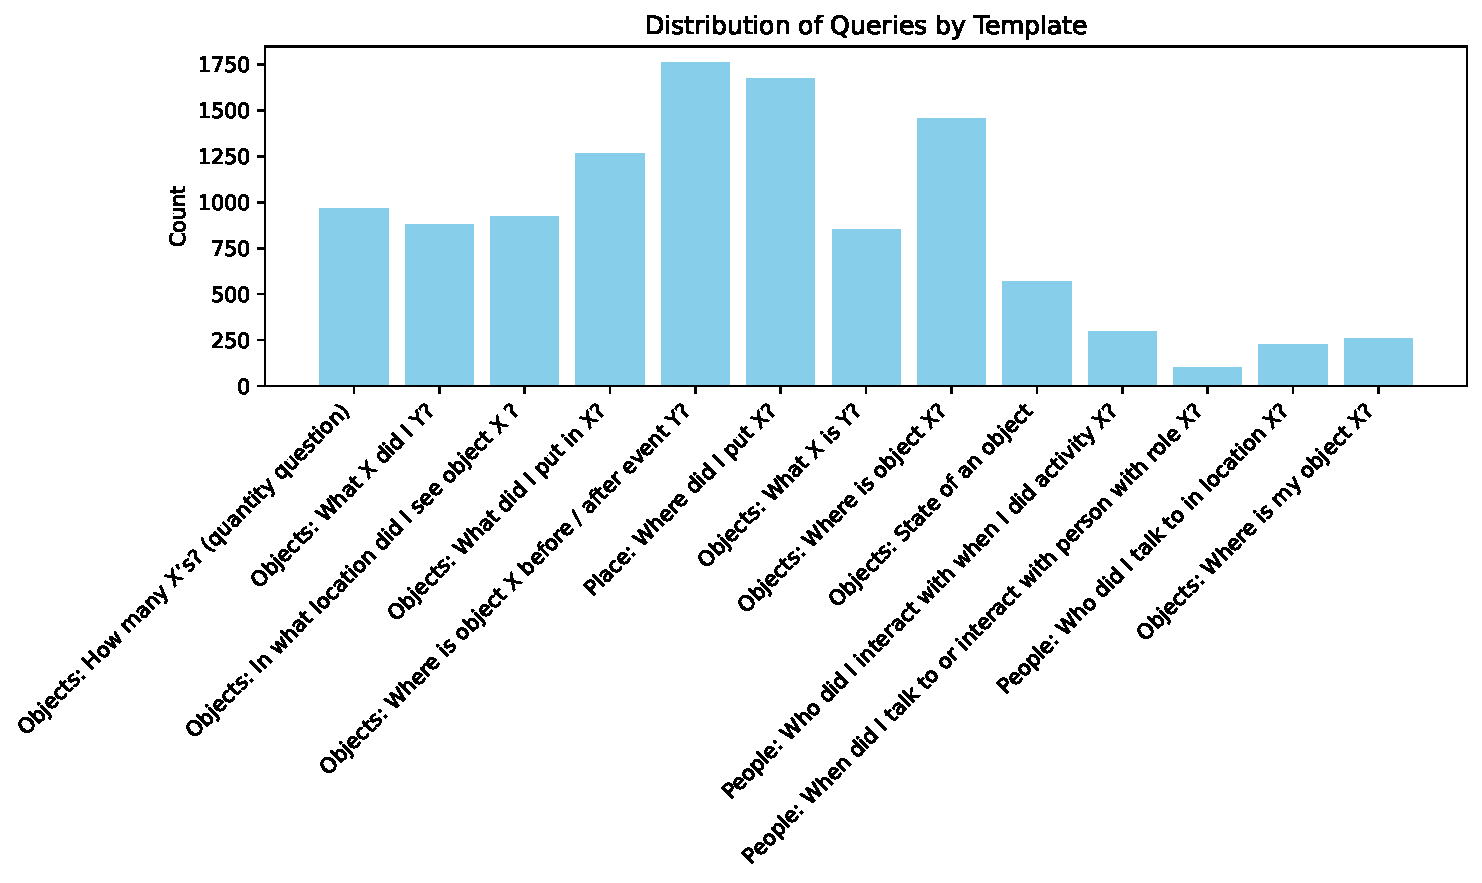
\includegraphics[height=4.5cm,width=0.48\textwidth]{Figure1.pdf} % adjust width as needed
\caption{Distribution of the number of queries for the different templates.}
\label{fig:figure1}
\end{figure}

Analyzing the data retrieved through annotations yields valuable insights for our current task. Initially, we note that the average duration of clips is 522 seconds, with the majority lasting 480 seconds (8 minutes). Approximately 9.01\% of the dataset consists of short queries, defined as lasting four frames or less at a frame rate of 30 frames per second; these queries of approximately 0 seconds duration are excluded.

Another observation from plotting the distribution is the relative duration of each query compared to the total duration of its corresponding video clip. Notably, most queries encompass 2\% or less of the total clip duration. To support this finding, we analyzed the average response interval and found it to be 9.67 seconds.

In fig. \ref{fig:figure2} reported below, we illustrate the distribution of the number of queries per video, suggesting an average of 15 queries per video.

\begin{figure}[h]
\centering
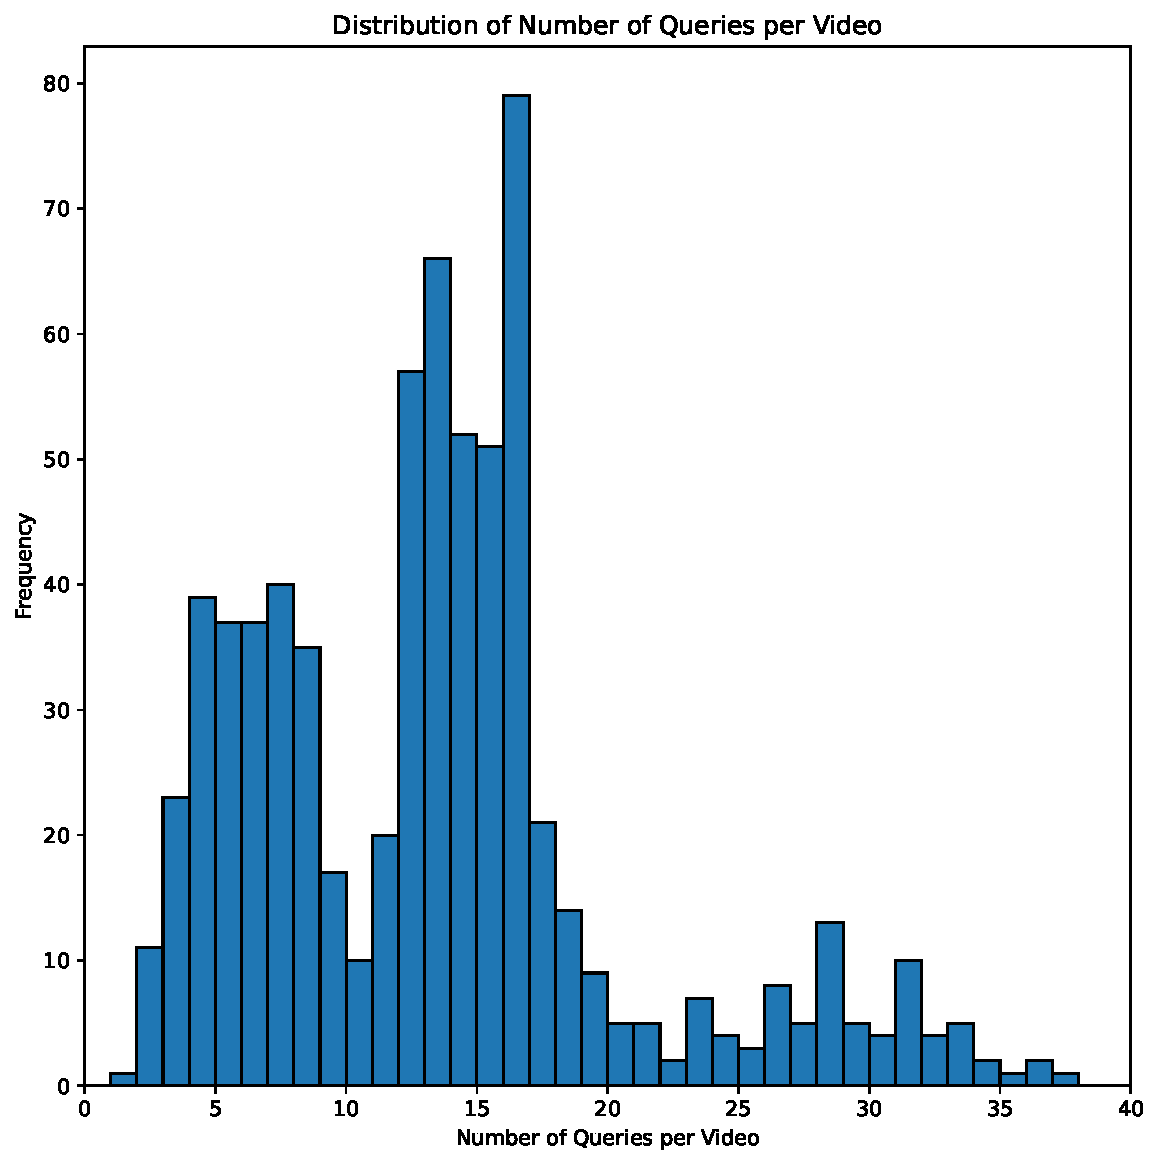
\includegraphics[width=0.36\textwidth]{Figure2.pdf} % adjust width as needed
\caption{Distribution of the number of queries for each video clip. Truncated for clarity, as the majority falls within the displayed range.}
\label{fig:figure2}
\end{figure}

Finally, it's interesting to note the correlation between each query and specific scenarios depicted in the video. Particularly, a significant number of queries (exceeding 100) are focused on the following scenarios: indoor navigation (walking), carpentry, cleaning/laundry, various jobs within construction and renovation companies (such as director of work, tiler, plumber, electrician, handyman, etc.), car mechanics, and cooking.


\section{Model architecture}

\begin{figure*}
  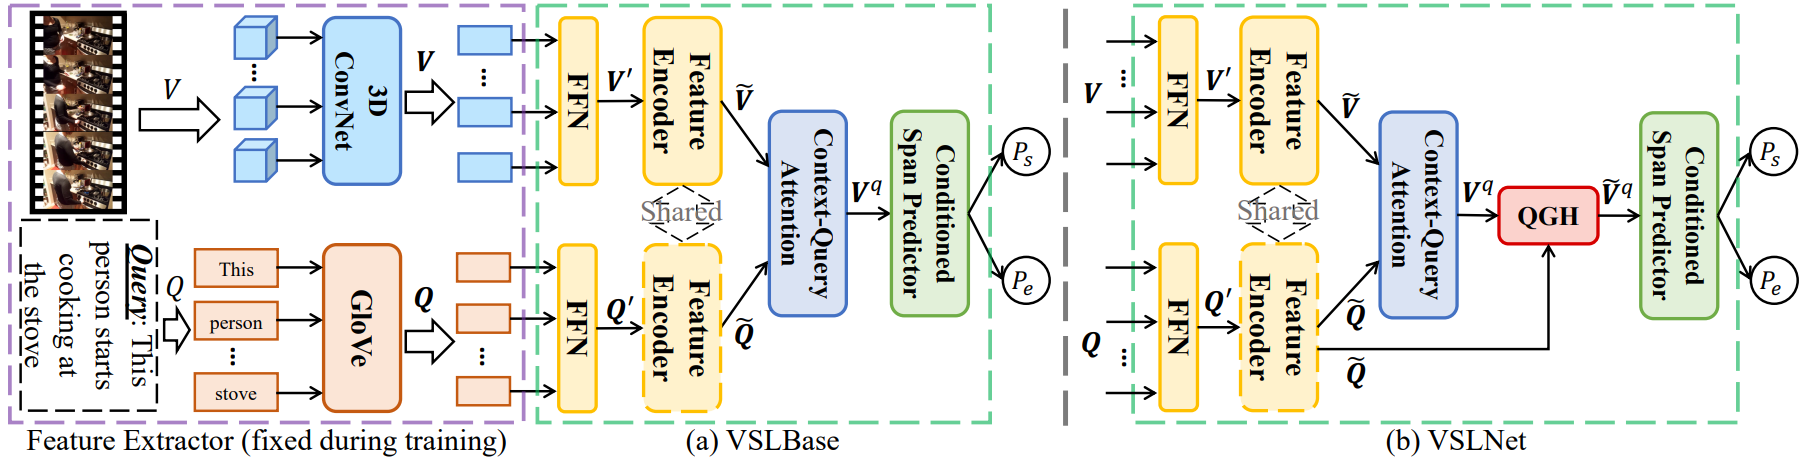
\includegraphics[width=\textwidth,height=4cm]{VSLnet.png}
  \caption{The two architectures for Natural Language Localization tasks are presented here. Figure (a) depicts the model architecture of VSLBase, while Figure (b) illustrates the model architecture of VSLNet.}
  \label{fig:VSL}
\end{figure*}

In this section, we delve into the architecture of the model, tracing its evolution from the first implementation to it subsequent enhancement through the integration of the Query-Guided Highlighting (QGH) module and the transition to the BERT encoder for query encoding, examining how these modifications contribute to the improvement of the performance of the model.

VSLBase (Fig. \ref{fig:VSL}a) is the first implementation of our model for video span localization, which leverages natural language queries to identify relevant segments within the video.  The model separately extracts visual and textual features from the inputted videos and queries. For the text query, GloVe word embedding is used to encode each word. GloVe provides a dense and fixed-size vector representation of the words in a high-dimensional space (300 dimensions in our case), capturing semantic similarities. Video features are extracted through a pre-trained convolutional neural network. In our case video features extraction was not computationally feasible, for this reason we employed pre-extracted video features instead (see paragraph 4.1). 

Once the features are extracted, they are projected into the same dimension by two linear layers. The projected features are then processed by a shared feature encoder, which consists of a series of convolutional and recurrent layers designed to refine and enhance the feature representations.

Next, the encoded features are aligned using an attention mechanism to capture their interaction. This context-query attention (CQA) mechanism computes relevance scores and attention weights for each video frame concerning the query, highlighting the segments of the video that are most likely to contain the answer.

Finally, this query-aware representation is fed into a conditioned span predictor that utilizes two stacked unidirectional Long Short-Term Memory networks (LSTMs) and two feed-forward layers for predicting start and end boundaries in the video context. The predictor computes the scores for start and end position, which are then normalized into probability distributions using a SoftMax function. During training, a crucial step for predicting the start and end boundaries of the target moment in a video is the computation of the training objective. The predicted probabilities are compared with the actual (ground truth) start and end positions using a cross-entropy loss. The results obtained are then averaged to obtain the Span loss.

To improve the performance of the VSLbase model, the QGH (Query-Guided Highlighting) module is introduced, leading to a more complete model, VSLNet (Fig. \ref{fig:VSL}b). In the pipeline, this module is placed after the CQA mechanism and before the span predictor module. The goal is to further highlight the features that are most important for the correct interval prediction.

An important part of the QGH module is the classification of the visual features obtained after the CQA step as either background or foreground. Using the query-aware representation, the process consists in computing the initial start and end boundaries of the target moment, considering these as the foreground while the rest of the features are considered background. Then, the boundaries of the foreground are extended before and after the initial predictions to add more context. The result of this process is a vector $Y_{h}$ that represents the classification of the features, where the ones in the background are marked as 0 while the ones in the foreground as 1.

Another core point of the module involves processing the query-aware representation obtained after the CQA mechanism and the word features obtained after encoding the query. Each visual feature is concatenated with an aggregated version of the query features. These new features are then used to compute the highlighting score $S_{h}$. This score is also an array where, for each feature, it represents the probability of being relevant for the prediction. By integrating this score with the visual features, we obtain a new representation of them that focuses even more on the most relevant ones for the prediction. This final representation is the input for the span predictors, which compute the results as described for the VSLbase model.

Finally, to complete the transition from VSLbase to the improved model, VSLNet, there is also a change in the loss function. The first part remains the same as in VSLbase, but an additional term, the cross-entropy loss between $Y_{h}$ and $S_{h}$, is added.

The last improvement to the model was done by substituting the GloVe embeddings with the BERT (Bidirectional Encoder Representations from Transformers) encoder, which allows for a deeper understanding of the query and subsequently a more context-aware representation of it.

The last improvement to the model was done by the substitution of the Glove embeddings with the BERT (Bidirectional Encoder Representations from Transformers) encoder that allow a deeper understanding of the query and subsequently a more context-aware representation of it.

\subsection{Pre-trained Features}
Due to the inaccessibility of the full 3,670 hours of Ego4D videos, we trained the model on precomputed features in a sliding window manner. Specifically, at each extraction point, the model processes the next window of size W frames (e.g., at frame i, the model sees features [i, i + W) frames). This window begins at frame 0 and slides with a specified stride until the end of the video [\href{https://ego4d-data.org/docs/data/features/}{Ego4D}]. We utilize slowfast8x8 as our baseline, and compare the outcomes with two other sets of precomputed features. A detailed overview of these features is presented in table \ref{tab:precomputedfeatures}.

\begin{table}[h]
\centering
\caption{Pre-computed Features for Ego4D}
\label{tab:precomputedfeatures}
\setlength{\tabcolsep}{4pt}
\renewcommand{\arraystretch}{1.2}
\resizebox{\linewidth}{!}{
\large
\begin{tabular}{@{}p{3cm}p{3cm}p{3cm}cc@{}}
\toprule
Feature Type & Dataset(s) Trained On & Model Arch & Window Size (W) & Stride \\
\midrule
SlowFast & Kinetics400 & SlowFast8x8\hspace{0.1cm}(R101 backbone) & 32 & 16 \\
Omnivore video & Kinetics400/ ImageNet-1K & Omnivore (Swin\hspace{0.1cm}L); video head & 32 & 16 \\
EgoVLP* & EgoClip/ HowTo100M & Frozen & 4 & 4 \\
\bottomrule
\end{tabular}
}

\begin{minipage}{\linewidth}
\vspace{0.1cm}  % Adjust spacing as needed
{\footnotesize * Note: The extraction process of EgoVLP was taken from \cite{egoVLP}.}  
\end{minipage}
\end{table}

\section{Proposed Approach}
\subsection{Task}
In the NLQ task, we use models that retrieve only the
information about the temporal interval of the video that
answers the input query, to return also a textual answer,
which could be more useful for the user, we need to use
Video Language Models(VLMs).\\
One problem of VLMs is that it is computationally expensive to process the entire video to answer the query. Therefore, we propose an approach that leverages the strengths of both type of models. We use a VslNet as first step of a pipeline to identify the short interval of interest. Then, we can cut the entire video to the interval of interest and feed it to a VLM alongside the query.
Another approach could be to aggregate the full video information to make it more feasible for the model. However, this could lead to a loss of detail.

The pipeline we used is shown in fig.\ref{fig:fullPipeline}, and for the VLM task, we chose Video-LLaVA.

\subsection{Video-LLava}
Video LLava is a Large Vision-Language model, so given a query and a visual input, its task is to produce a textual answer.  It is capable of simultaneously handling both image and videos. Many existing approaches encode images and videos into separate input spaces, but this can be a limitation. Instead, this model uses a unified visual representation for both modalities within the language feature space.\\
Also, in paper \cite{b8} it is shown that unified visual representation befits LLMs in learning both images and videos when compared to models specifically designed for one of the modalities.
\subsubsection{Model Structure}
The first step consists in extracting visual features (from videos or images). For this purpose, LanguageBind encoders are used \cite{b9}. These encoders can map different modalities into the textual feature space. At the end of this process, we obtain a unified visual representation.\\ 
The next step is to use a shared projection layer to project the features, then they are in the same space with the tokenized textual queries. We can then input all the data into a large LLM to get the answer.\\
A key point of Video LLaVA is the alignment of visual modalities before projection. LanguageBind naturally aligns image and language in shared feature space using pretrained encoders. To align video representation to the language space it uses 3 millions video-text pairs from VIDAL-10M\cite{b9}. Therefore, before projection, data from both modalities are in a unified feature space.

\subsubsection{Training pipeline}
After obtaining the tokenized version of the textual input and visual signals input, the training consists in an optimization problem, that lead the model to achieve multi-modal understanding capabilities.
This means that for each prediction in the training set, the objective is to maximize the probability of returning the ground-truth output based on the given input textual and visual tokens. \\
An important point to note at this stage, which is also one of the model's strengths, is the simultaneous training on both images and videos, with every batch containing both types of data.\\
In the first stage of training, the main focus is on associating the textual data with visual data using a extensive image/video-text pair dataset.\\
The second phase is the instruction tuning, the objective is still an optimization problem but with the addition of a context variable. The context is the combination of the previous queries and answers.\\
Thus, at this stage, this model is trained to answer to more than one instruction. It must produce an output for several sequential and more complex queries, taking into consideration the entire conversation.
(Non mi sembra importante ma at this stage also the LLM are involved in training)

\begin{figure*}
  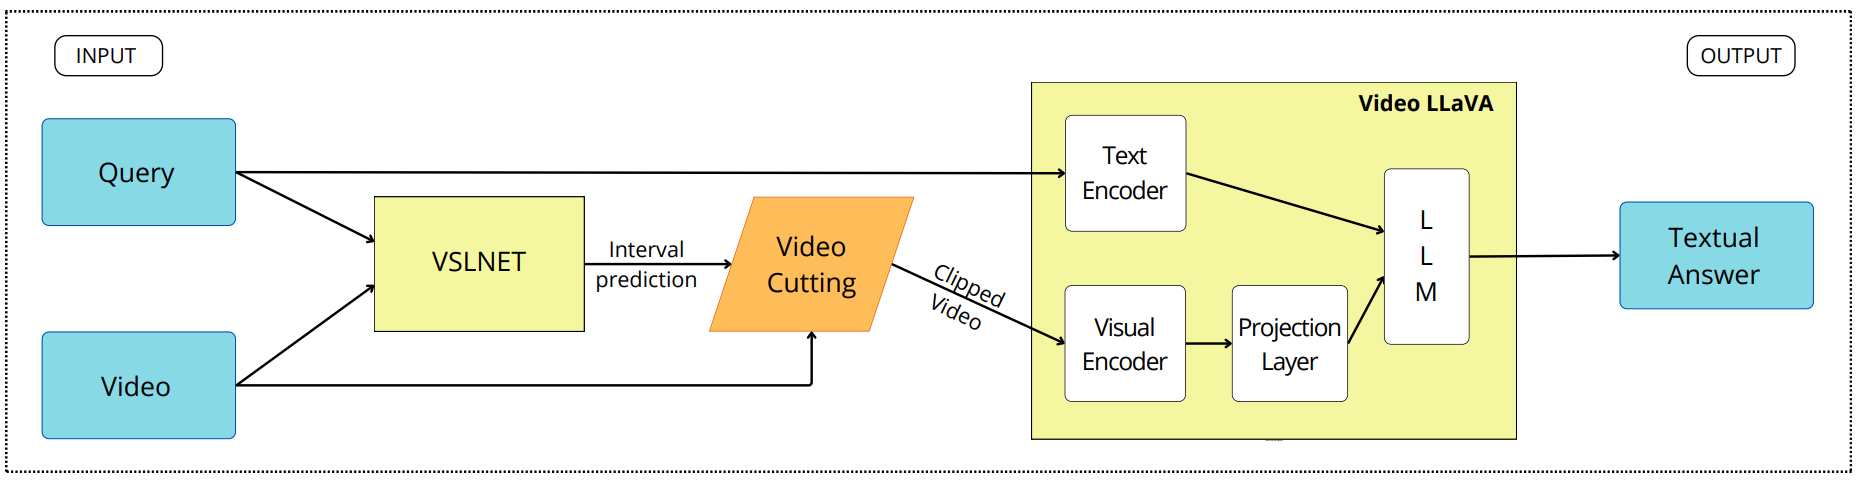
\includegraphics[width=\textwidth,height=4cm]{FinalProposedPipeline.png}
  \caption{The figure depicts the complete pipeline, from the inputted video and queries to the generation of the answer, encompassing the architecture of Video-LLaVA.}
  \label{fig:fullPipeline}
\end{figure*}

\subsection{Parameters}
\label{subsec:Parameters}
During our tests we also observed the behaviour of the model bychanging some parameters related to output, the tested parameters were:

\begin{itemize}
\setlength{\parskip}{0.05cm} 
    \item \textit{\textbf{Max Length}}: it controls the lenght of the produced answer
    \item \textit{\textbf{Temperature}}: it controls the "creativity" of the answer, for high values, at each step, it flattens the probability distribution used to select the next word, so it can happen that the model selects also words with a lower probability score during the sequence generation, this could results in more creative but also less accurate answer
    \item \textit{\textbf{Top K}}: similarly to temperature, it also controls the diversity of the output, during the sequence generation, at each step, the model sample from the top K most probable textual tokens, higher value of K means higher diversity but also less accuracy
    \item \textit{\textbf{Top P}}: it controls the balance between accuracy and diversity, at each step, for the sampling are chosen the smallest number of tokens that have a cumulative probability greater or equal to P
     \item \textit{\textbf{Num Beam}}: it controls the number of sequence that the model maintains at each step, an higher number can lead to more accurate solution. Basically at every iteration the algorithm try to combine to the current sequences with all the possible words, after doing that, the probability of all the new sequences is computed and the $Num Beam$ most probable sequences are kept for the following step
    
\end{itemize}

\section{Results}
In this section, we discuss the results obtained by our proposed pipeline. The results are divided into two parts, the first one presents the numerical evaluation of the NLQ task and the scores obtained by the textual answers produced by VideoLLaVA on several tests. The second part is a qualitative assessment, as it is not possible to judge the results of textual answers referring only to the score.

\subsection{Numerical Results}
\subsubsection{NLQ task}
The metrics that we took into consideration to compare the obtained results are the following:
\begin{itemize}
    \item \textit{\textbf{IoU}}, Intersection over Union(IoU), it is the proportion between the intersection and the union of the ground-truth and predicted intervals\\
    \begin{equation}
    \hspace{-0.5cm}
        IoU = \frac{\text{PredictedInterval} \cap \text{Ground-TruthIntverval}}{\text{PredictedInterval} \cup \text{Ground-TruthIntverval}}
    \end{equation}
    \item \textit{\textbf{r@k}}, Recall at rank k (r@k) is used to measure how high the correct interval is positioned in the ranking of a prediction. %For example, r@1 indicates the percentage of predictions where the correct interval is ranked as the most probable solution.
    This metric is usefull because, for each query, multiple intervals are identified as possible solutions, and these intervals are ranked based on how well the model considers them to match the query
\end{itemize}
\vspace{-0.3cm}
\begin{table}[h]
\centering
\small 
\caption{NLQ Performance}
\label{tab:performance}
\begin{tabular}{@{}p{2.4cm}p{1.0cm}lcccccc@{}}
\toprule
\multirow{2}{*}{Model} & \multirow{2}{*}{Features} & \multicolumn{2}{c}{IoU=0.3 (\%)} & \multicolumn{2}{c}{IoU=0.5 (\%)} \\ 
& & r@1  & r@5 & r@1   & r@5       \\ \midrule
VSLNet\hspace{0.2mm}(Baseline) & SlowFast & 5.45 & 10.74 & 3.12 & 6.63 \\ 
VSLNet & Omnivore & 6.48 & 14.04 & 3.72 & 8.70 \\ 
VSLNet & EgoVlp & 8.03 & 15.82 & 4.75 & 10.12 \\ 
VSLBase & Omnivore & 6.58 & 13.37 & 3.56 & 8.60 \\
VSLBase & EgoVlp & 7.18 & 14.74 & 4.26 & 9.65 \\
VSLNet* & Omnivore & 3.05 & 8.36 & 1.21 & 4.34 \\
VSLNet* & EgoVlp & 3.79 & 9.53 & 2.17 & 5.83 \\
\bottomrule
\end{tabular}
\captionsetup{font=footnotesize}
\caption*{VSLNet* is the version that uses GloVe as encoder instead of BERT.}
\end{table}

From the table, considering the cases in which the BERT encoder is used, we can notice that both VSLNet and VSLBase, using Omnivore and EgoVLP as pre-extracted features, perform better than VSLNet using SlowFast. It is important to specify that this improvement could also be due to the fact that annotations and features might have been updated since the publication of the original baseline in the paper.
\\
In particular, VSLNet with EgoVlp features significantly outperforms the others when we consider $IoU = 0.3$ and $r@1$, as well as when $IoU = 0.5$ and $r@5$.
\\
Models that do not use BERT as an encoder perform significantly worse than those that do. This could be because the BERT encoder is more sophisticated, indeed, it also takes into account the context in which words are used.

\subsubsection{Extension evaluation}
For the VLM task evaluation we decided to use the following metrics:
\begin{itemize}
    \item \textit{\textbf{R-F1}}: ROUGE-1 F1 Score(R-F1) is related to to overlap between the predicted sentence and the ground-truth. Computed as $F1-Score$ using the following precision and recall: 
    \begin{equation*}
        Precision = \frac{\text{\small Number of overlapping words}}{\text{ \small Total words in the prediction}}
    \end{equation*}
     \begin{equation}
        Recall = \frac{\text{\small Number of overlapping words}}{\text{\small Total words in the ground truth}}
    \end{equation}
    \item \textit{\textbf{METEOR}}: The METEOR score is a more comprehensive metric than ROUGE. METEOR, similarly to ROUGE, produces a score between 0 and 1, however, precision and recall are computed after an alignment process that includes stemming and synonyms matching.
    \item \textit{\textbf{B-F1}}, The BERT F1 Score(B-F1) is as an advanced evaluation metric because it incorporates contextual understanding. It utilizes pre-trained contextual embeddings from BERT to compare the embeddings of the prediction sentence and ground truth sentence, measuring their similarity with cosine similarity. After this process it is possible to compute the recall, precision and F1 score(B-F1).
\end{itemize}

\begin{table}[h]
\centering
\caption{VLM Performance}
\label{tab:comparisonSCore}
\begin{tabular}{@{}lccc@{}}
\toprule
Configuration & R F1 & Meteor & B-F1 \\ \midrule
Default & 0.59 & 0.53 & 0.93 \\
Temperature 10.0 & 0.42 & 0.38 & 0.90 \\
TopP 0.3 & 0.63 & 0.59 & 0.94 \\
Beam 2 & 0.52 & 0.53 & 0.92 \\
Max Length 10 & 0.54 & 0.44 & 0.91 \\
TopK 200 & 0.44 & 0.42 & 0.90\\
\bottomrule
\end{tabular}
\captionsetup{font=footnotesize}
\caption*{Each configuration name represents the parameter we modified with the new value from the default settings.}
\end{table}

In table \ref{tab:comparisonSCore} we show the score obtained, using models with some parameters variations.
The default parameters were:

\begin{itemize}
\footnotesize  % or \small for a slightly larger size
\itemsep=0.1cm    
    \item {$Temperature = 1.0$}
    \item {$Num Beam = 1$}
    \item {$Top K = 2$}
    \item {$Top P = 0.9$}
    \item {$Max new tokens = 100$}
\end{itemize}

We have done multiple test on the parameters mentioned in \ref{subsec:Parameters}. Here, we present the results obtained using the default parameters, the configuration that achieved the best and worst performances were, respectively, those with $Top P = 0.3$ and the one with $Temperature = 10$. Additionally, in the table we reported the results obtained with the furthest variation of the parameters from default values.\
Notably, for both R-F1 and Meteor metrics, no configuration achieved results as good as those obtained with the best configuration. Probably, $Top P = 0.3$ obtains the highest scores, because it produces human-like predictions that are semantically close to our ground truth. When examining the B-F1 scores, we observe that they are generally higher and more consistent across different configurations. This is because B-F1 assesses similarity based on semantic similarity, regardless of exact phrasing. Consequently, Bert's scores are usually high even when the predictions do not exactly match the ground truth.
\\
The previous consideration was more focused on the sentences semantic, if we talk about the accuracy of the predictions made by Video-LLaVA, the results is show below. To do this evaluation we had to manually chek if the answers was correct, since the score values do not reflect the correctness. The total number of predictions was 50, we split them based on their category shown in \ref{fig:figure1}. We illustrate the performance of the proposed approach among different categories.
Since the generated answers changed at every run, we computed an average of three prediction sets:

\begin{itemize}
\itemsep=0.1cm  
\small
    \item overall, we have a 30\% success rate, with an average of 15 correctly answered queries over a total of 50 queries.
    \item for the Objects category we have a 24\% success rate, with an average of 10 correctly answered queries over a total of 42.
    \item for the Place category we have a 11\% success rate, with an average of 0.67 query over a total of 6.
    \item for the People category we have a 100\% success rate, but on only 2 queries.   
\end{itemize}

\subsection{Qualitative Results}
In our study, visualizing the input video can help assessing the model's capacity to provide well-reasoned responses. Below, we present some of the most intriguing qualitative results we obtained. These results imply that the model performs well in cases that call for descriptive responses, providing insights that are quite similar to answers that have been manually annotated.

A first example is illustrated in fig. \ref{fig:animation1}, the model successfully identified the object in question (broccoli) despite a brief clip that lacked clear information. In this case, the model's response surpassed our observation, since we mistakenly identified the object as green peppers. If considering the entire video, it becomes evident that the correct identification is the one provided by the algorithm.

To confirm the efficiency of the model, we reported further results where the model correctly identifies the subjects of interest, available at \href{https://github.com/Gin549/episodic-memory-pers/tree/main/qualitative_results}{this link}.

\begin{figure}[ht]
  \centering
  \animategraphics[autoplay,loop, height=4.2cm]{12}{BroccoliClip/output_}{0001}{0055}
  \captionsetup{justification=centering} % Center the caption
  \caption{\textbf{Query}: \textit{What vegetables did I chop?} \\\textbf{Answer}: \textit{You chopped a head of lettuce and a piece of broccoli on the cutting board.}}
  \label{fig:animation1}
\end{figure}


However, the model presents limitations in specific tasks, particularly in counting objects or when asked to provide precise quantities. Figure \ref{fig:animation2} exemplifies this: the model was inquired to identify the exact number of fuse holders picked from a box. The ground truth indicated six fuse holders, but the model mistakenly numbered two. This discrepancy may be attributed to the fact that the individual in the video is holding only two fuse holders in their left hand at the end of the video, and the algorithm may struggle with maintaining a precise knowledge of the temporal sequence of activities.
The inaccuracy in counting extends to several other queries, with additional examples available at the link mentioned above.
\begin{figure}[ht]
  \centering
  \animategraphics[autoplay,loop, height=4.2cm]{12}{FuseHoldClip/output_}{0001}{0068}
  \captionsetup{justification=centering} % Center the caption
    \caption{\textbf{Query}: \textit{How many fuse holders did I pick from the box?} \\\textbf{Answer}: \textit{You picked two fuse holders from the box.}}
  \label{fig:animation2}
\end{figure}


Furthermore, we observed that the model frequently provides erroneous answers to yes/no questions. We highlight this issue in fig. \ref{fig:animation3}, where the model provides a wrong answer despite the video clearly showing the action. One assumption is that in these situations, when the model has to choose between two options for the initial token, there is a greater chance that it will select the incorrect term. This can be due to the limitation of a binary choice, where any slight bias can significantly impact the final decision. Systematic mistakes may also result from a skewed internal probability distribution for "yes" and "no" tokens in the training data.

\begin{figure}[ht]
  \centering
  \animategraphics[autoplay,loop, height=4.2cm]{12}{TapClip/output_}{0001}{0130}
  \captionsetup{justification=centering} % Center the caption
      \caption{\textbf{Query}: \textit{Did I leave the tap open?} \\\textbf{Answer}: \textit{Yes, you left the tap open in the sink.}}
  \label{fig:animation3}
\end{figure}

\section{Conclusions}
Throughout our analysis we have proposed and evaluated an advanced pipeline addressing the NLVL challenge working with two state-of-the-art models. By combining the strenght of VSLNet for precise video segment localization and Video-LLAva for generating accurate textual answers,we have demonstrated how these innovations improved traditional methods.
We have proved that our pipeline achieves good performances overall, although there are some areas where the model falls short, thereby indicating where future work should focus in order to reach an even higher accuracy.
We had the chance to see that despite the strong performance in many scenarios, the model struggles with very complex queries or poorly formulated ones, highlighting a potential area for improvement in robustness to variations in input quality.
%------------------------------------------------------------------------

%%%%%%%%% REFERENCES
{\small
\bibliographystyle{ieee_fullname}
\bibliography{egbib}
}
\end{document}
